
%\documentclass[a4paper,11pt,twoside]{ThesisStyle}
\documentclass[a4paper,11pt,twoside]{article}

\title{Answer to the second round of comments from the Ad-hoc review committee \\
 Measurement of deeply virtual Compton
scattering off Helium-4 with CLAS at Jefferson Lab}


\date{\today}
\usepackage{amsmath,amssymb}             % AMS Math
% \usepackage[french]{babel}
\usepackage[latin1]{inputenc}
\usepackage[OT1]{fontenc}
\usepackage[left=2.7cm,right=1.7cm,top=1.6cm,bottom=1.6cm,includefoot,includehead,headheight=13.6pt]{geometry}
\usepackage{setspace}
\usepackage{epigraph}
\usepackage{lineno}


%\usepackage{arev}
%\usepackage[bitstream-charter]{mathdesign}
%\usepackage[urw-garamond]{mathdesign}
%\usepackage[sfmath]{kpfonts} %% sfmath option only to make math in sans serif. Probablye only for use when base font is sans serif.
%\renewcommand*\familydefault{\sfdefault} %% Only if the base font of the document is to be sans serif
\usepackage[sc]{mathpazo}
\linespread{1.05}   
\usepackage[T1]{fontenc}



% Table of contents for each chapter

\usepackage[nottoc, notlof, notlot]{tocbibind}
\usepackage{minitoc}
\setcounter{minitocdepth}{2}
\mtcindent=15pt
% Use \minitoc where to put a table of contents

\usepackage{aecompl}

% Glossary / list of abbreviations

\usepackage[intoc]{nomencl}
\renewcommand{\nomname}{List of Abbreviations}

\makenomenclature

% My pdf code

\usepackage{graphicx,type1cm,eso-pic,color}
\usepackage{lscape}

  \usepackage[pagebackref,hyperindex=true]{hyperref}

%\geometry{letterpaper}
%\graphicspath{{.}{images/}}

% nicer backref links
\renewcommand*{\backref}[1]{}
\renewcommand*{\backrefalt}[4]{%
\ifcase #1 %
(Not cited.)%
\or
(Cited on page~#2.)%
\else
(Cited on pages~#2.)%
\fi}
\renewcommand*{\backrefsep}{, }
\renewcommand*{\backreftwosep}{ and~}
\renewcommand*{\backreflastsep}{ and~}

% Links in pdf
\usepackage{color}
\definecolor{linkcol}{rgb}{0,0,0.4} 
\definecolor{citecol}{rgb}{0.5,0,0} 

% Change this to change the informations included in the pdf file

% See hyperref documentation for information on those parameters

\hypersetup
{
bookmarksopen=true,
pdftitle="",
pdfauthor="", pdfsubject="", %subject of the document
%pdftoolbar=false, % toolbar hidden
pdfmenubar=true, %menubar shown
pdfhighlight=/O, %effect of clicking on a link
colorlinks=true, %couleurs sur les liens hypertextes
pdfpagemode=None, %aucun mode de page
pdfpagelayout=SinglePage, %ouverture en simple page
pdffitwindow=true, %pages ouvertes entierement dans toute la fenetre
linkcolor=linkcol, %couleur des liens hypertextes internes
citecolor=citecol, %couleur des liens pour les citations
urlcolor=linkcol %couleur des liens pour les url
}

% definitions.
% -------------------

\setcounter{secnumdepth}{3}
\setcounter{tocdepth}{2}

% Some useful commands and shortcut for maths:  partial derivative and stuff
\newcommand{\xbp}{$x_{Bj}$}
\newcommand{\xb}{$x_{Bj}~$}
\newcommand{\ptp}{$p_\perp^2$}
\newcommand{\pt}{$p_\perp^2~$}
\newcommand{\dptp}{$\Delta \langle p_\perp^2 \rangle$}
\newcommand{\dpt}{$\Delta \langle p_\perp^2 \rangle ~$}

\brokenpenalty10000\relax

\newcommand{\pd}[2]{\frac{\partial #1}{\partial #2}}
\def\abs{\operatorname{abs}}
\def\argmax{\operatornamewithlimits{arg\,max}}
\def\argmin{\operatornamewithlimits{arg\,min}}
\def\diag{\operatorname{Diag}}
\newcommand{\eqRef}[1]{(\ref{#1})}

\usepackage{rotating}                    % Sideways of figures & tables
%\usepackage{bibunits}
%\usepackage[sectionbib]{chapterbib}          % Cross-reference package (Natural BiB)
%\usepackage{natbib}                  % Put References at the end of each chapter
                                         % Do not put 'sectionbib' option here.
                                         % Sectionbib option in 'natbib' will do.
\usepackage{fancyhdr}                    % Fancy Header and Footer

% \usepackage{txfonts}                     % Public Times New Roman text & math font
  
%%% Fancy Header %%%%%%%%%%%%%%%%%%%%%%%%%%%%%%%%%%%%%%%%%%%%%%%%%%%%%%%%%%%%%%%%%%
% Fancy Header Style Options

\pagestyle{fancy}                       % Sets fancy header and footer
\fancyfoot{}                            % Delete current footer settings

%\renewcommand{\chaptermark}[1]{         % Lower Case Chapter marker style
%  \markboth{\chaptername\ \thechapter.\ #1}}{}} %

%\renewcommand{\sectionmark}[1]{         % Lower case Section marker style
%  \markright{\thesection.\ #1}}         %

\fancyhead[LE,RO]{\bfseries\thepage}    % Page number (boldface) in left on even
% pages and right on odd pages
\fancyhead[RE]{\bfseries\nouppercase{\leftmark}}      % Chapter in the right on even pages
\fancyhead[LO]{\bfseries\nouppercase{\rightmark}}     % Section in the left on odd pages

\let\headruleORIG\headrule
\renewcommand{\headrule}{\color{black} \headruleORIG}
\renewcommand{\headrulewidth}{1.0pt}
\usepackage{colortbl}
\arrayrulecolor{black}

\fancypagestyle{plain}{
  \fancyhead{}
  \fancyfoot{}
  \renewcommand{\headrulewidth}{0pt}
}

%\usepackage{algorithm}
%\usepackage[noend]{algorithmic}

%%% Clear Header %%%%%%%%%%%%%%%%%%%%%%%%%%%%%%%%%%%%%%%%%%%%%%%%%%%%%%%%%%%%%%%%%%
% Clear Header Style on the Last Empty Odd pages
\makeatletter

\def\cleardoublepage{\clearpage\if@twoside \ifodd\c@page\else%
  \hbox{}%
  \thispagestyle{empty}%              % Empty header styles
  \newpage%
  \if@twocolumn\hbox{}\newpage\fi\fi\fi}

\makeatother
 
%%%%%%%%%%%%%%%%%%%%%%%%%%%%%%%%%%%%%%%%%%%%%%%%%%%%%%%%%%%%%%%%%%%%%%%%%%%%%%% 
% Prints your review date and 'Draft Version' (From Josullvn, CS, CMU)
\newcommand{\reviewtimetoday}[2]{\special{!userdict begin
    /bop-hook{gsave 20 710 translate 45 rotate 0.8 setgray
      /Times-Roman findfont 12 scalefont setfont 0 0   moveto (#1) show
      0 -12 moveto (#2) show grestore}def end}}
% You can turn on or off this option.
% \reviewtimetoday{\today}{Draft Version}
%%%%%%%%%%%%%%%%%%%%%%%%%%%%%%%%%%%%%%%%%%%%%%%%%%%%%%%%%%%%%%%%%%%%%%%%%%%%%%% 

\newenvironment{maxime}[1]
{
\vspace*{0cm}
\hfill
\begin{minipage}{0.5\textwidth}%
%\rule[0.5ex]{\textwidth}{0.1mm}\\%
\hrulefill $\:$ {\bf #1}\\
%\vspace*{-0.25cm}
\it 
}%
{%

\hrulefill
\vspace*{0.5cm}%
\end{minipage}
}

\let\minitocORIG\minitoc
\renewcommand{\minitoc}{\minitocORIG \vspace{1.5em}}

\usepackage{multirow}
%\usepackage{slashbox}

\newenvironment{bulletList}%
{ \begin{list}%
	{$\bullet$}%
	{\setlength{\labelwidth}{25pt}%
	 \setlength{\leftmargin}{30pt}%
	 \setlength{\itemsep}{\parsep}}}%
{ \end{list} }

\newtheorem{definition}{D�finition}
\renewcommand{\epsilon}{\varepsilon}

% centered page environment

\newenvironment{vcenterpage}
{\newpage\vspace*{\fill}\thispagestyle{empty}\renewcommand{\headrulewidth}{0pt}}
{\vspace*{\fill}}



\begin{document}

\maketitle

\section*{}
Having discussed your second draft and replies to our comments, we are satisfied on all points except 2 and 5.
We'll start with the minor quibble. \\

\textbf{Point 5} \\
You have left the sentence: \textit{"Its historic use to measure DVCS in many different configurations made it an ideal
place for this new DVCS measurement."} Our objection is mostly focused on the word "ideal," which connotes
"perfection." (Also historic is not quite the word you want.) You have explained what you mean to communicate,
and so we urge you to write: \textit{"It was naturally well-suited for measuring DVCS, and several DVCS experiments
were successfully conducted using multiple different configurations."} \\
   \textcolor{blue}{Text has been changed.}

\textbf{Point 2:} \\
Our remaining concern is still on the subtraction of background coming from exclusive $\pi^0$ s with a missing photon.
Your response was helpful in correcting some of our misunderstandings. We think this is a complicated point
because the problem is nested.
\begin{enumerate}
\item There is the BSA in the $\pi^0$ production itself.
\item There is the possibility of an apparent BSA in the $\phi$ distribution that you reconstruct from the single detected
photon, when you are forced to (incorrectly) assume that the process is DVCS.
\item There is the change in BSA that happens as a part of the subtraction of the $\pi^0$ background.
\end{enumerate}
Let us address each.
\begin{enumerate}
\item The use of a $\pi^0$ generator with no BSA is an interesting analysis choice. I don't think it's our committee's job
to critique that choice. It's clear that the MC does a good job of reproducing incoherent exclusive $\pi^0$ data
(your Fig. 15) so the choice is well-motivated. It's interesting that this contrasts with a measured BSA in
exclusive $\pi^0$ production on a proton. You haven't given us enough to understand whether your data could
see 5-10\% BSA. We think it's your choice how deep you want to go when discussing that in the paper. We'd
prefer more discussion, but that's your choice to make. \\
   \textcolor{blue}{The very thorough analysis of F. Cao on the coherent $\pi^0$ channel (with the same data) indicates that no BSA is detectable in the coherent channel. It also shows we could probably resolve a BSA if it was around 10\% or more, but not around 5\%. We can assume these error levels are similar in the incoherent channel even though no detailed analysis exists there. We had some discussions with the group behind this other analysis and they want to make an independent paper, so we do not want to "steal" their figures. However, if the committee feels we should clarify some of the text, we are happy to add some sentences on the topic. But, we would need clearer guidance on what information you would like us to add.}
\item You have pointed out that Figs. 14 and 15 show good agreement between the $\pi^0$ simulation and the measured
$\pi^0$ data. But this doesn't answer our concern about what the distribution of $\pi^0$ single photon events looks
like when binned according to the $\phi$ you would use when you assume the event is DVCS. Your simulation
can answer that question. It seems like that distribution is what really matters when assessing a false BSA
coming from $\pi^0$ s. Are we being naive in asking that? Is guaranteed to be flat for some reason that we don't
understand? \\
   \textcolor{blue}{Previously, we understood your question to be about the generated $\pi^0$, these are flat in $\phi$ and thus, the photons from their decay as well. However, the single photons from $\pi^0$ making it into the DVCS sample are modified by the acceptance of CLAS and follow a different distribution. We do not have a figure for this, but it can be easily reconstructed from the two plots in Fig. \ref{fig}. One can multiply the histogram on the left with the ratio on the right to get the detected single photons from $\pi^0$. As we can see things are almost flat on the right and the distribution will be very similar to the one from fully reconstructed $\pi^0$.}
\item It's not clear what (if any) correction you are making to your reported BSA. You write:
\textit{"to make the correction on the DVCS BSA, . . .} \\
 $[$implying you are making a correction$]$ \\
   \textcolor{blue}{We have to disagree here, we do not imply we make a correction, we are saying it.} \\
\textit{. . . we assume that the exclusive $\pi^0$ production has no such asymmetry. . . .} \\
 $[$fine, but that's not the relevant $\phi$ angle!$]$ \\
   \textcolor{blue}{If there is no BSA in the  $\pi^0$ production, we do not see how changing angle could generate some BSA. Our impression is that this would only be relevant if we used a non-0 BSA.} \\
\textit{. . . This has been checked with the exclusive $\pi^0$ production data for which no significant level of BSA was
measured."} \\
\end{enumerate}
This still leaves questions un-answered for the reader. For the committee to be happy to approve this paper, we
would like:
\begin{itemize}
\item The sentence about the BSA to be made more clear. Are you making a correction for $\pi^0$ contamination? Are
you not making a correction? How big is the correction to the BSA you extract? \\
  \textcolor{blue}{We do not see how this text is ambiguous as to the fact that we apply a correction. The correction is described over about 20 lines, 3 figures and 2 equations. It is unclear to us what could make the reader think that we do not apply the correction described. The size of the correction is given in the figure 16, we are unsure what more you are asking.}
\item Some response (doesn't have to go in the paper) about what the simulated distribution of $\pi^0$ events with a
missing photon looks like, when binned in the $\phi$ that you calculate assuming DVCS. Is it flat? Is there a fake
BSA? Is there some reason why we are naive to think that this is important? We need to know more to assess
whether or not what you have written is clear and accurate. \\
  \textcolor{blue}{The first part of this question is answered above and illustrated with Fig. \ref{fig}. On the second part of the question, we do not see how a fake BSA can be generated from a process without any BSA in the first place. It is very difficult to answer this question as you ask to know more, but you are not saying about what. If you want to know more about the correction, you can read the text in the analysis note on this topic. If that is still unclear we are happy to discuss in a meeting or to answer questions as above that point at specific issues that are unclear.}
\end{itemize}
A $\phi$ distribution of the A LU before and after the correction for the $N_{1\gamma,\pi^0}$ contamination would go a long way
to satisfy everyone on the issue of $\pi^0$ background in the incoherent case.\\
 \textcolor{blue}{ We do not have this figure at hand and it would take a while to produce. However, it can be again more or less estimated thanks to existing figures that this correction has very little $\phi$ dependence as DVCS and $\pi^0$ have similar distributions (illustrated in Fig. \ref{fig}). } \\

 \textcolor{blue}{Some final comments on this question of the $\pi^0$ correction. The bin with the largest $\pi^0$ contamination is 17\%, so assuming a 10\% BSA from free proton data, that would lead to a 1.7\% change on our DVCS BSA result in this bin (much less elsewhere). A few comments on this: (i) this is accounted for in our systematic errors and falls well within our error bars; (ii) both nuclear effects and the fact that we measure only a single photon would reduce the size of the BSA actually getting in our measurement compared to a free proton target, so a 1.7\% effect is even an exaggerated figure; (iii) this change would be reducing the $\pi^0$ correction we apply as it would make the $\pi^0$ events more like the DVCS events; (iv) therefore, such change in the analysis would reduce our final DVCS BSA; (v) our main conclusion on the incoherent is that the incoherent DVCS asymmetries are unexpectedly low already, so the discussed change if implemented would not weaken our conclusions it would reinforce them (by a fraction of $\sigma$). For all these reasons, we do think this correction does not necessitate an in depth reanalysis as we are performing now or a much more detailed description in the paper.}

\begin{figure}[htbp!]
\center
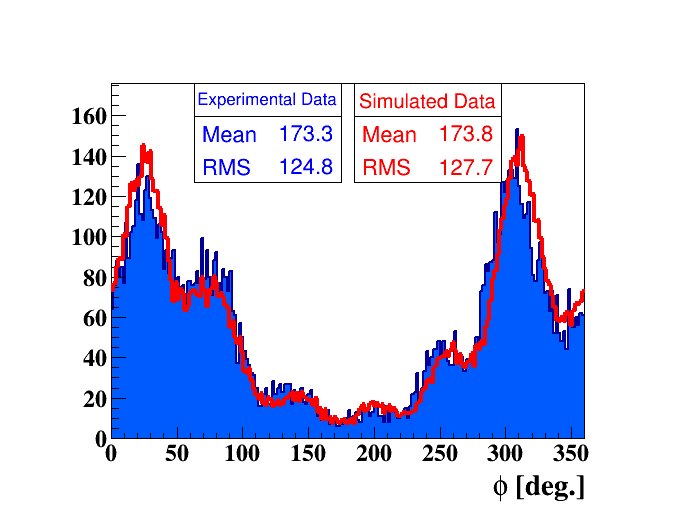
\includegraphics[width=8.2cm]{../../../analysis-note-vf/fig_dvcs/comp/phi_h_InCoh_pi0.png}
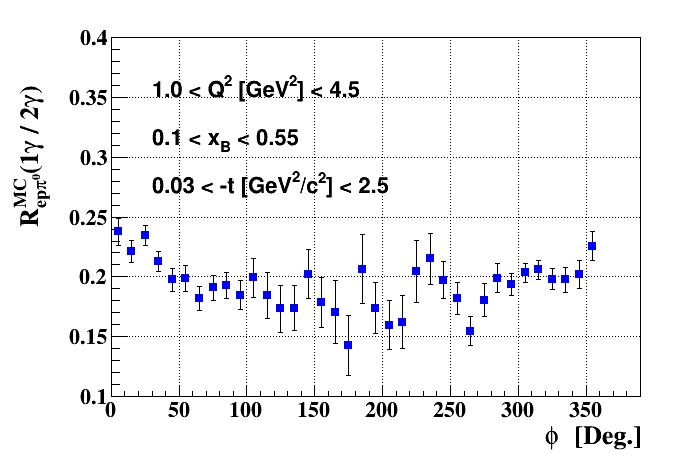
\includegraphics[width=8.2cm]{../../../analysis-note-vf/fig_dvcs/epgamma_eppi0_Phi.png}
\caption{Left, the distribution of $\pi^0$ measured (blue) and simulated (red). Right, the ratio of DVCS like single photon events from $\pi^0$ to detectable 2 photons $\pi^0$ events.}
\label{fig}
\end{figure}

\end{document}
